\documentclass{article}
\usepackage{hyperref}
\usepackage{graphicx}
\begin{document}
\title{CrossCorr parameter space double-cone \\ 
LIGO-T1600313}
\author{Grant David Meadors}
\date{\today}
%\affiliation{AEI Hannover/Golm}

\maketitle

CrossCorr's 3D parameter space (frequency $f$, projected semi-major axis $a \sin i$, time of ascension $t_\mathrm{asc}$) includes a double-cone structure around simulated signals. 
On this cone, test statististc $\rho$ values are significantly higher than background, but less than the maximum. 
This structure can be considered a long-range correlation. 
While the metric approximation should not be expected to hold on the cone, the cone equation is derivable from degeneracies in the signal model. 
We illustrate this equation with figures and compare results to the corresponding $X$-pattern found in TwoSpect.

\section{Introduction}



The theory makes more sense now, and I have more and better graphs.


Following Ansel's suggestion, I mimicked the TwoSpect injection from the
original post,

\begin{figure}
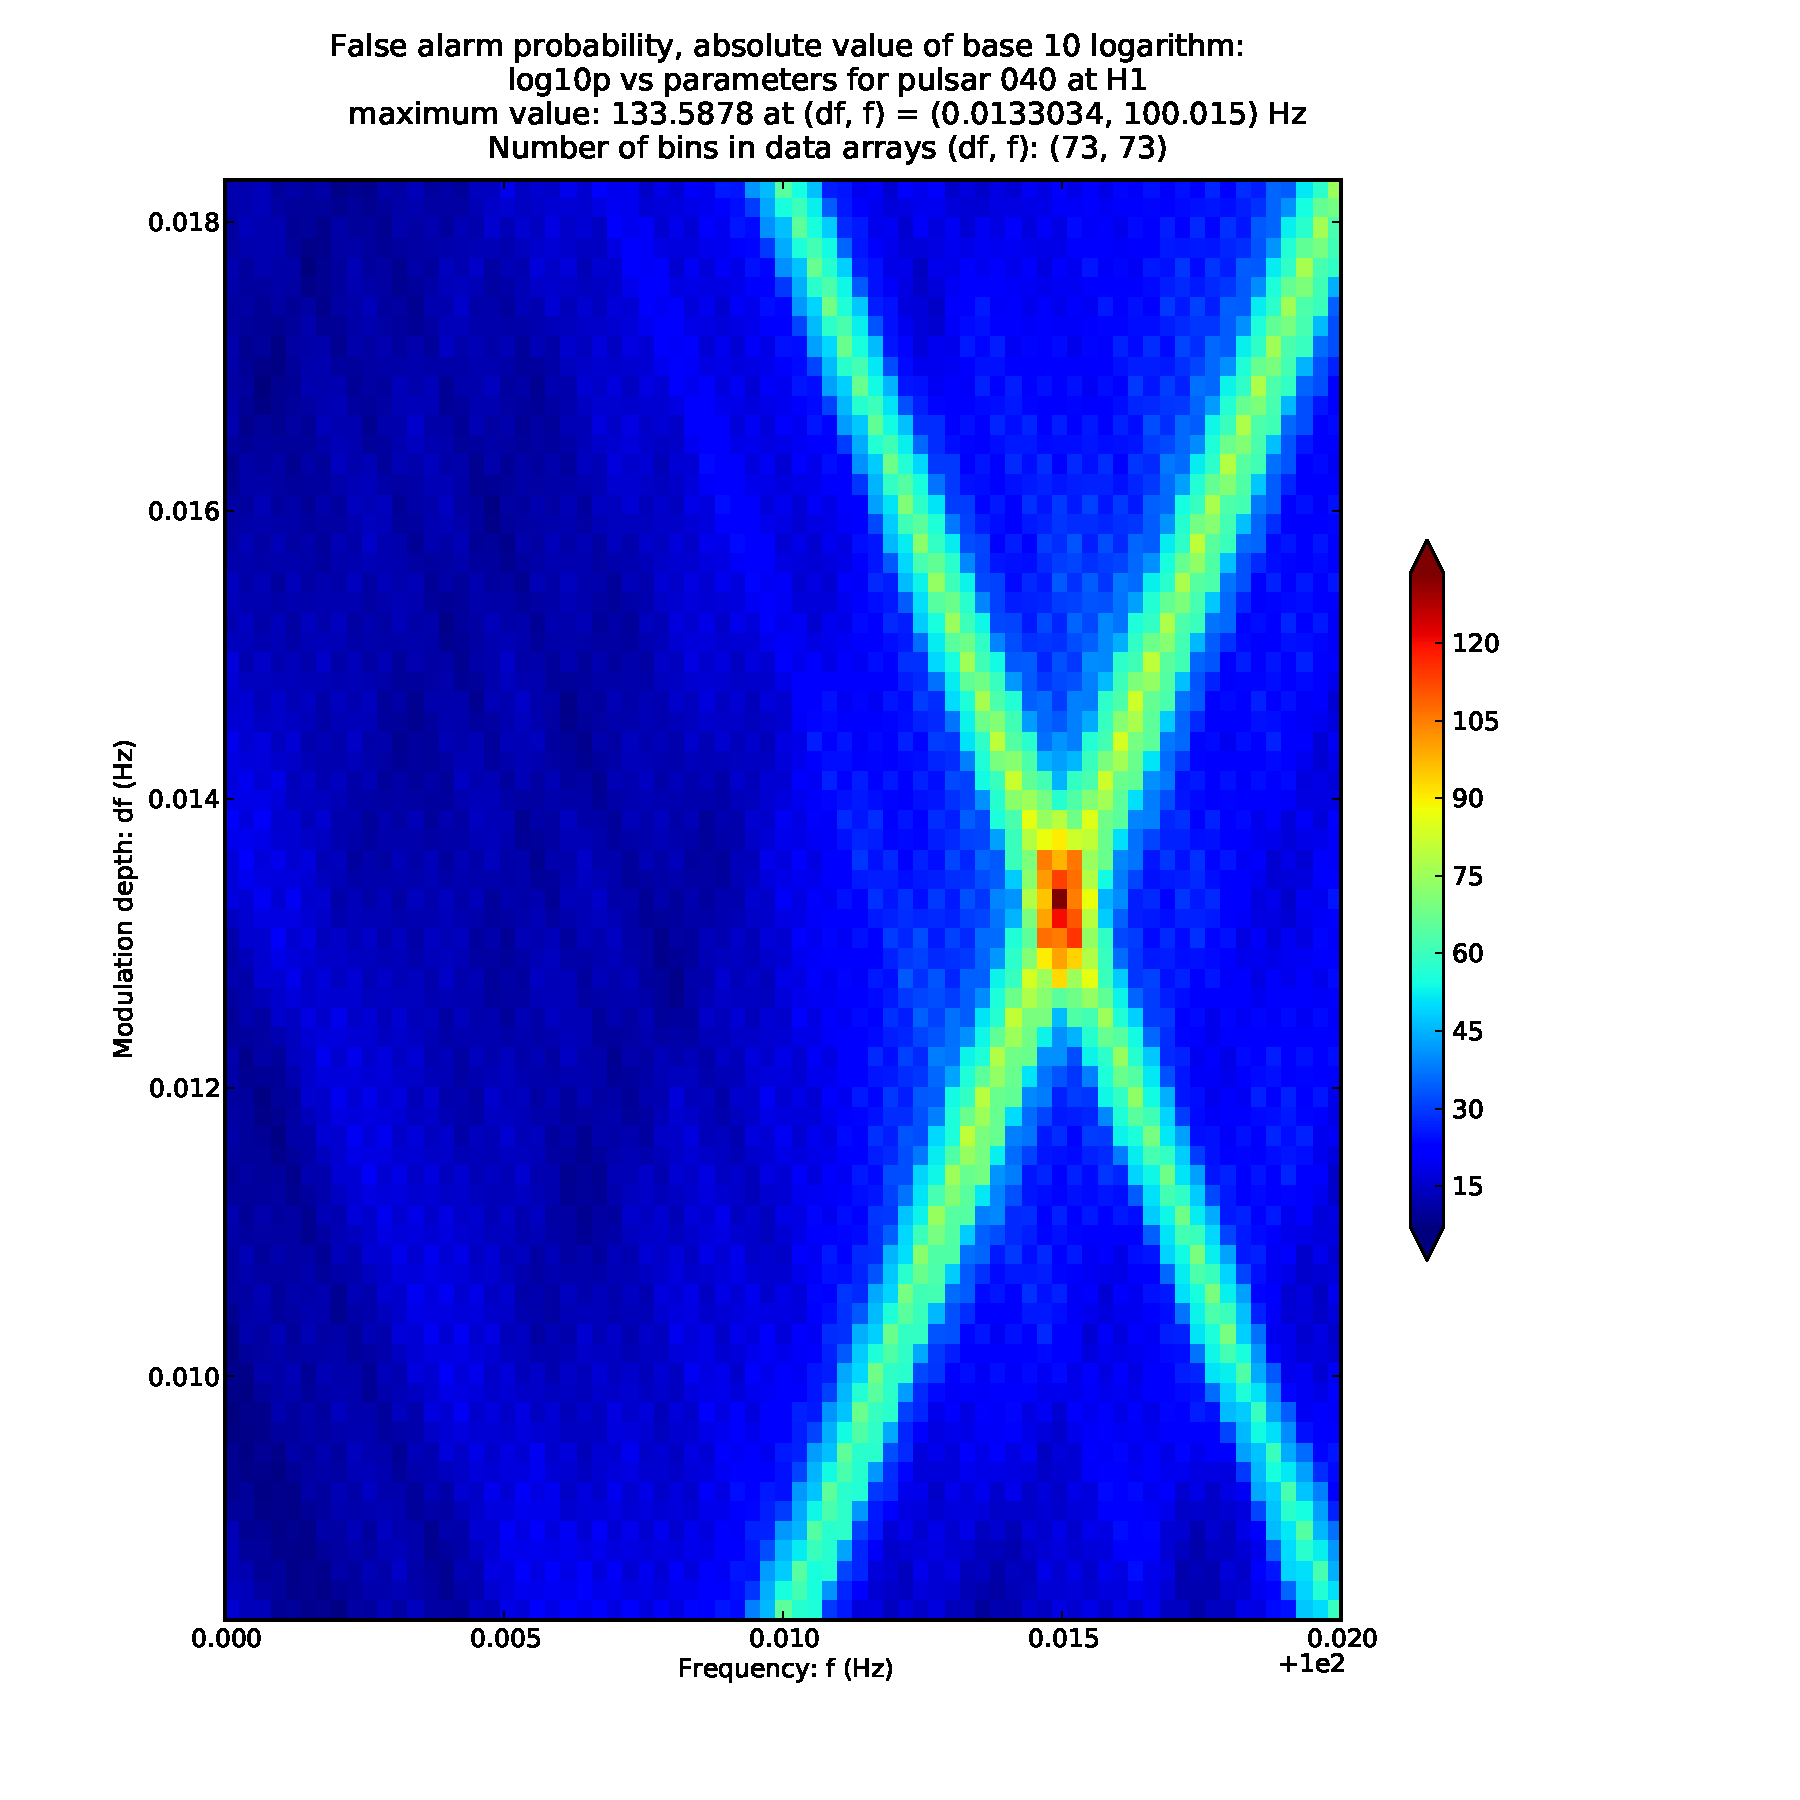
\includegraphics[trim= 0 0 0 0, clip, width=0.40\paperwidth,keepaspectratio]{plots/DFvsFresultsProb-H1_pulsar-040.pdf}
\caption{
\url{<
https://ldas-jobs.ligo-wa.caltech.edu/~gmeadors/TwoSpect/2014/06/18/injections/graph-H1-40e-26-TSni/DFvsFresultsProb-H1_pulsar-040.pdf
>}
}
\end{figure}

with CrossCorr ($T_sft$ = 840 s, \texttt{maxLag} = 840 s). The full set of commands
(run as in "example-TwoSpect-like.txt"; log in "\texttt{log\_crosscorr.txt}") and
Python scripts is in, with some duplication,

\begin{center}
\url{<
https://www.atlas.aei.uni-hannover.de/~grant.meadors/LSC/ScoX1/2016/07/21-CrossCorr/
>}
\end{center}

Note for CrossCorr people: I'm plotted the (modulation depth = 2 pi a
sin i / P) dimension instead of a sin i, but the script allows either.

Walking through it, I've taken 2D slices through the
frequency-modulation depth, modulation depth-time of ascension, and time
of ascension-frequency planes. F = "frequency", A = "modulation depth"
(~"a sin i"), T="time of ascension"; each slice preserves F-A-T cyclic
order.

Slices through the injection center:

\begin{figure}
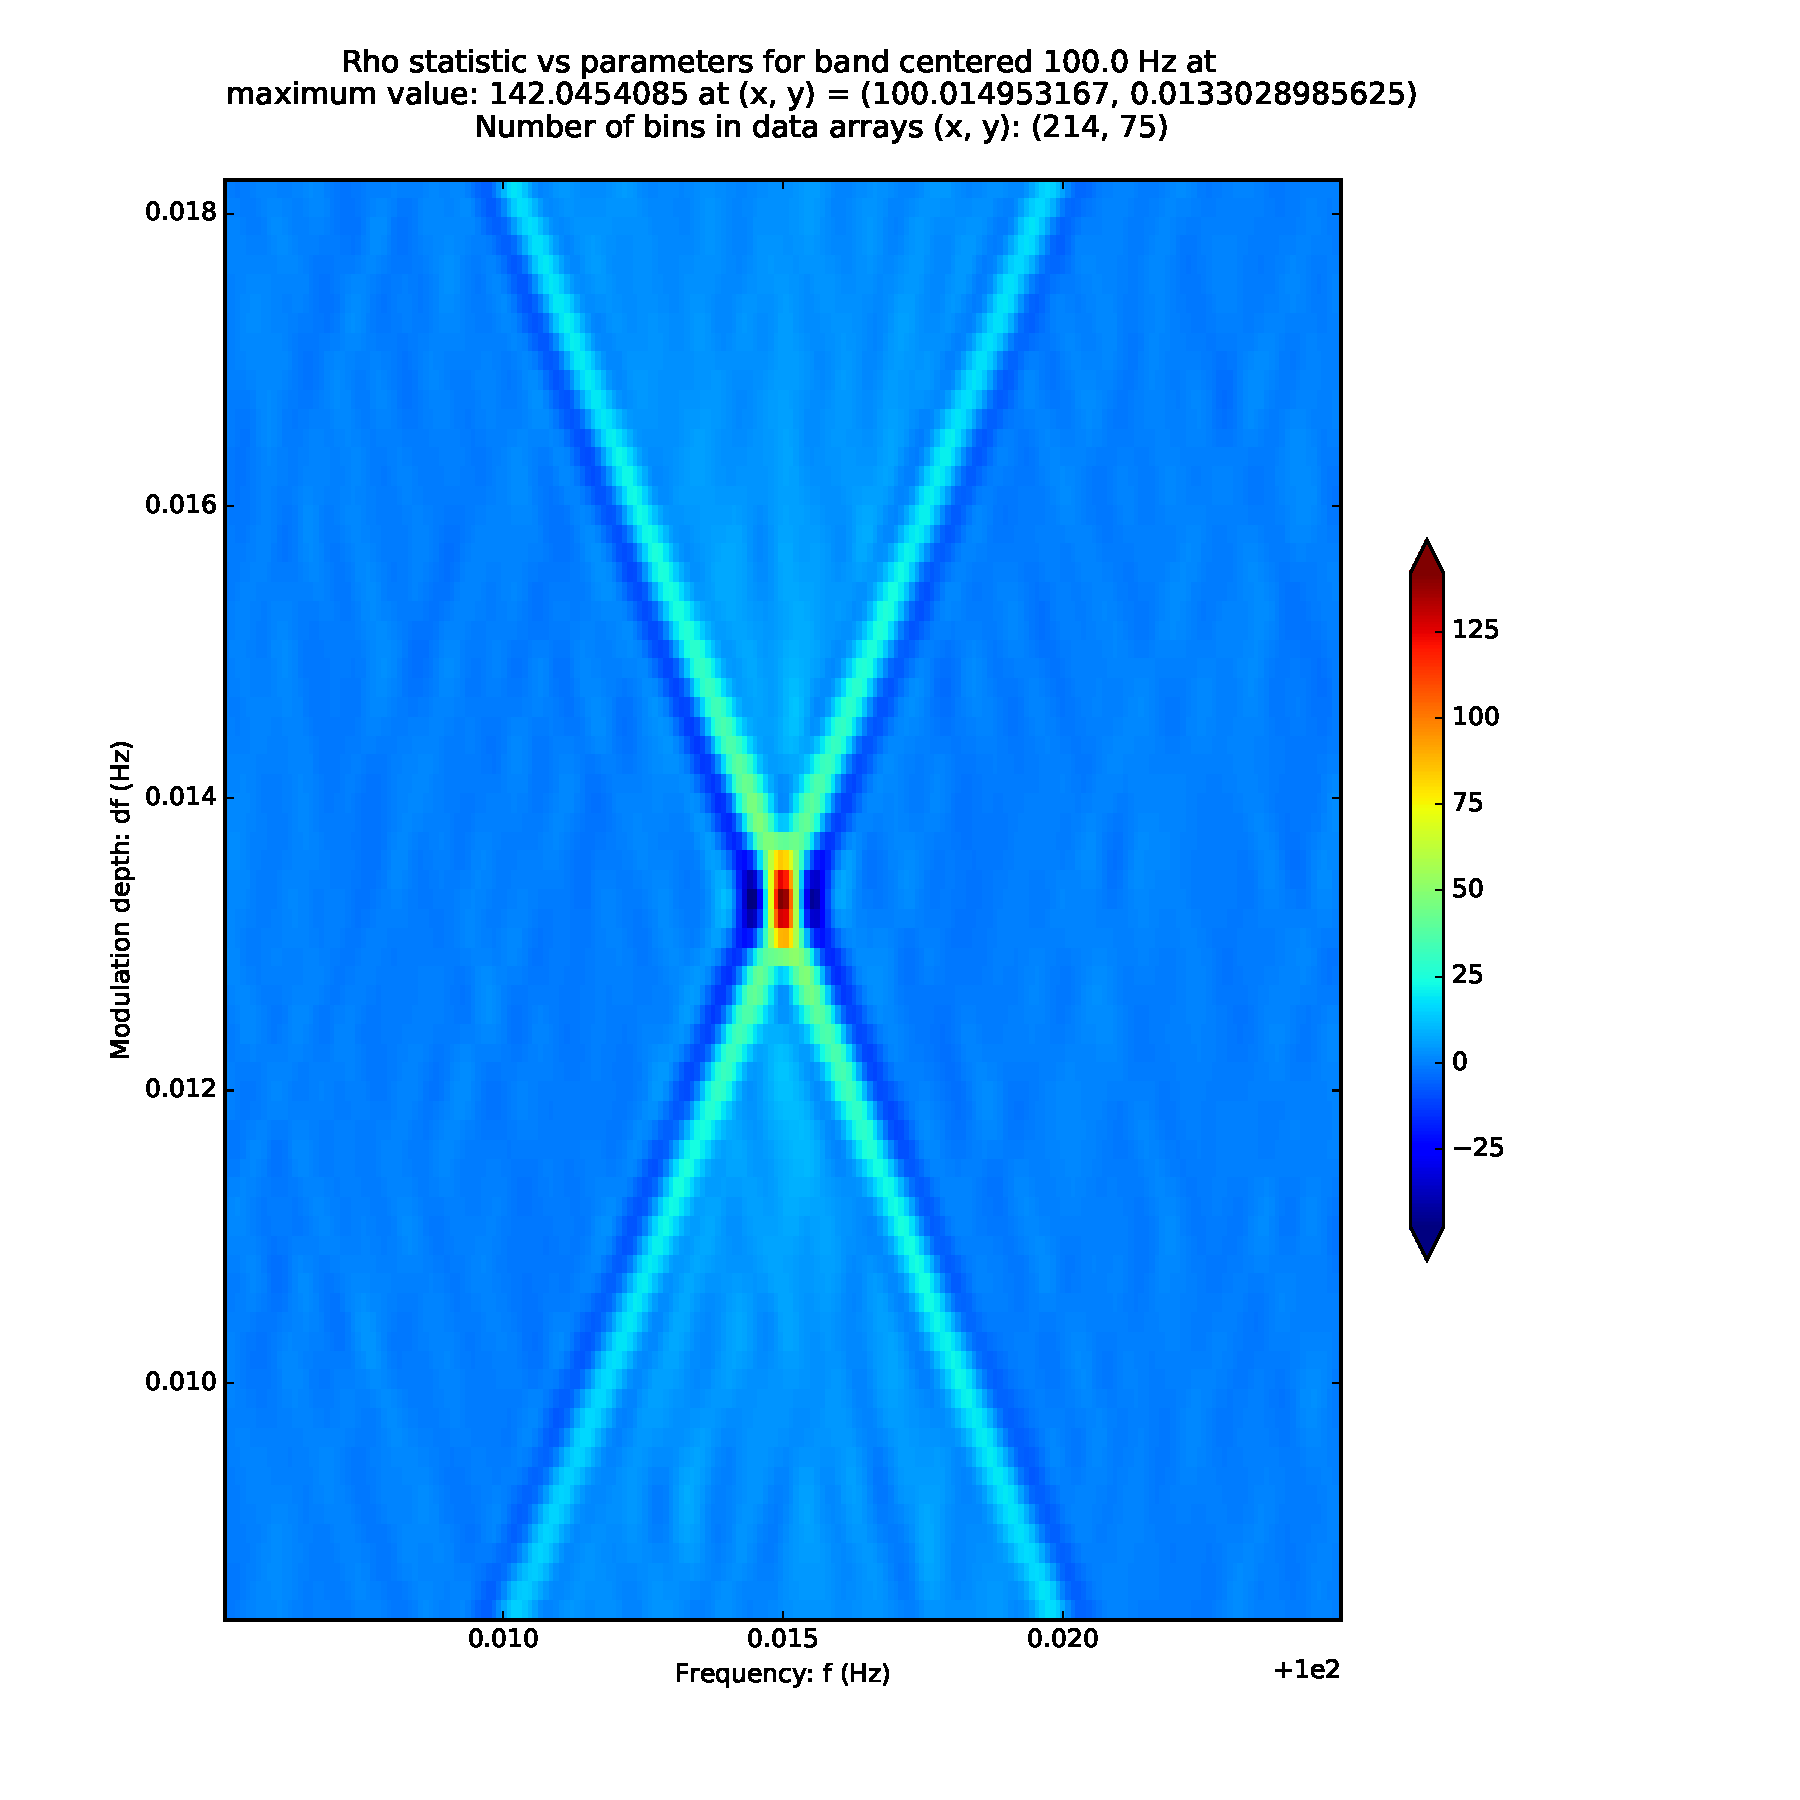
\includegraphics[trim= 0 0 0 0, clip, width=0.40\paperwidth,keepaspectratio]{plots/match-TS/FAresultsR-band-100-0.pdf}
\caption{
\url{<
https://www.atlas.aei.uni-hannover.de/~grant.meadors/LSC/ScoX1/2016/07/21-CrossCorr/match-TS/FAresultsR-band-100.0.pdf
>}
}
\end{figure}

\begin{figure}
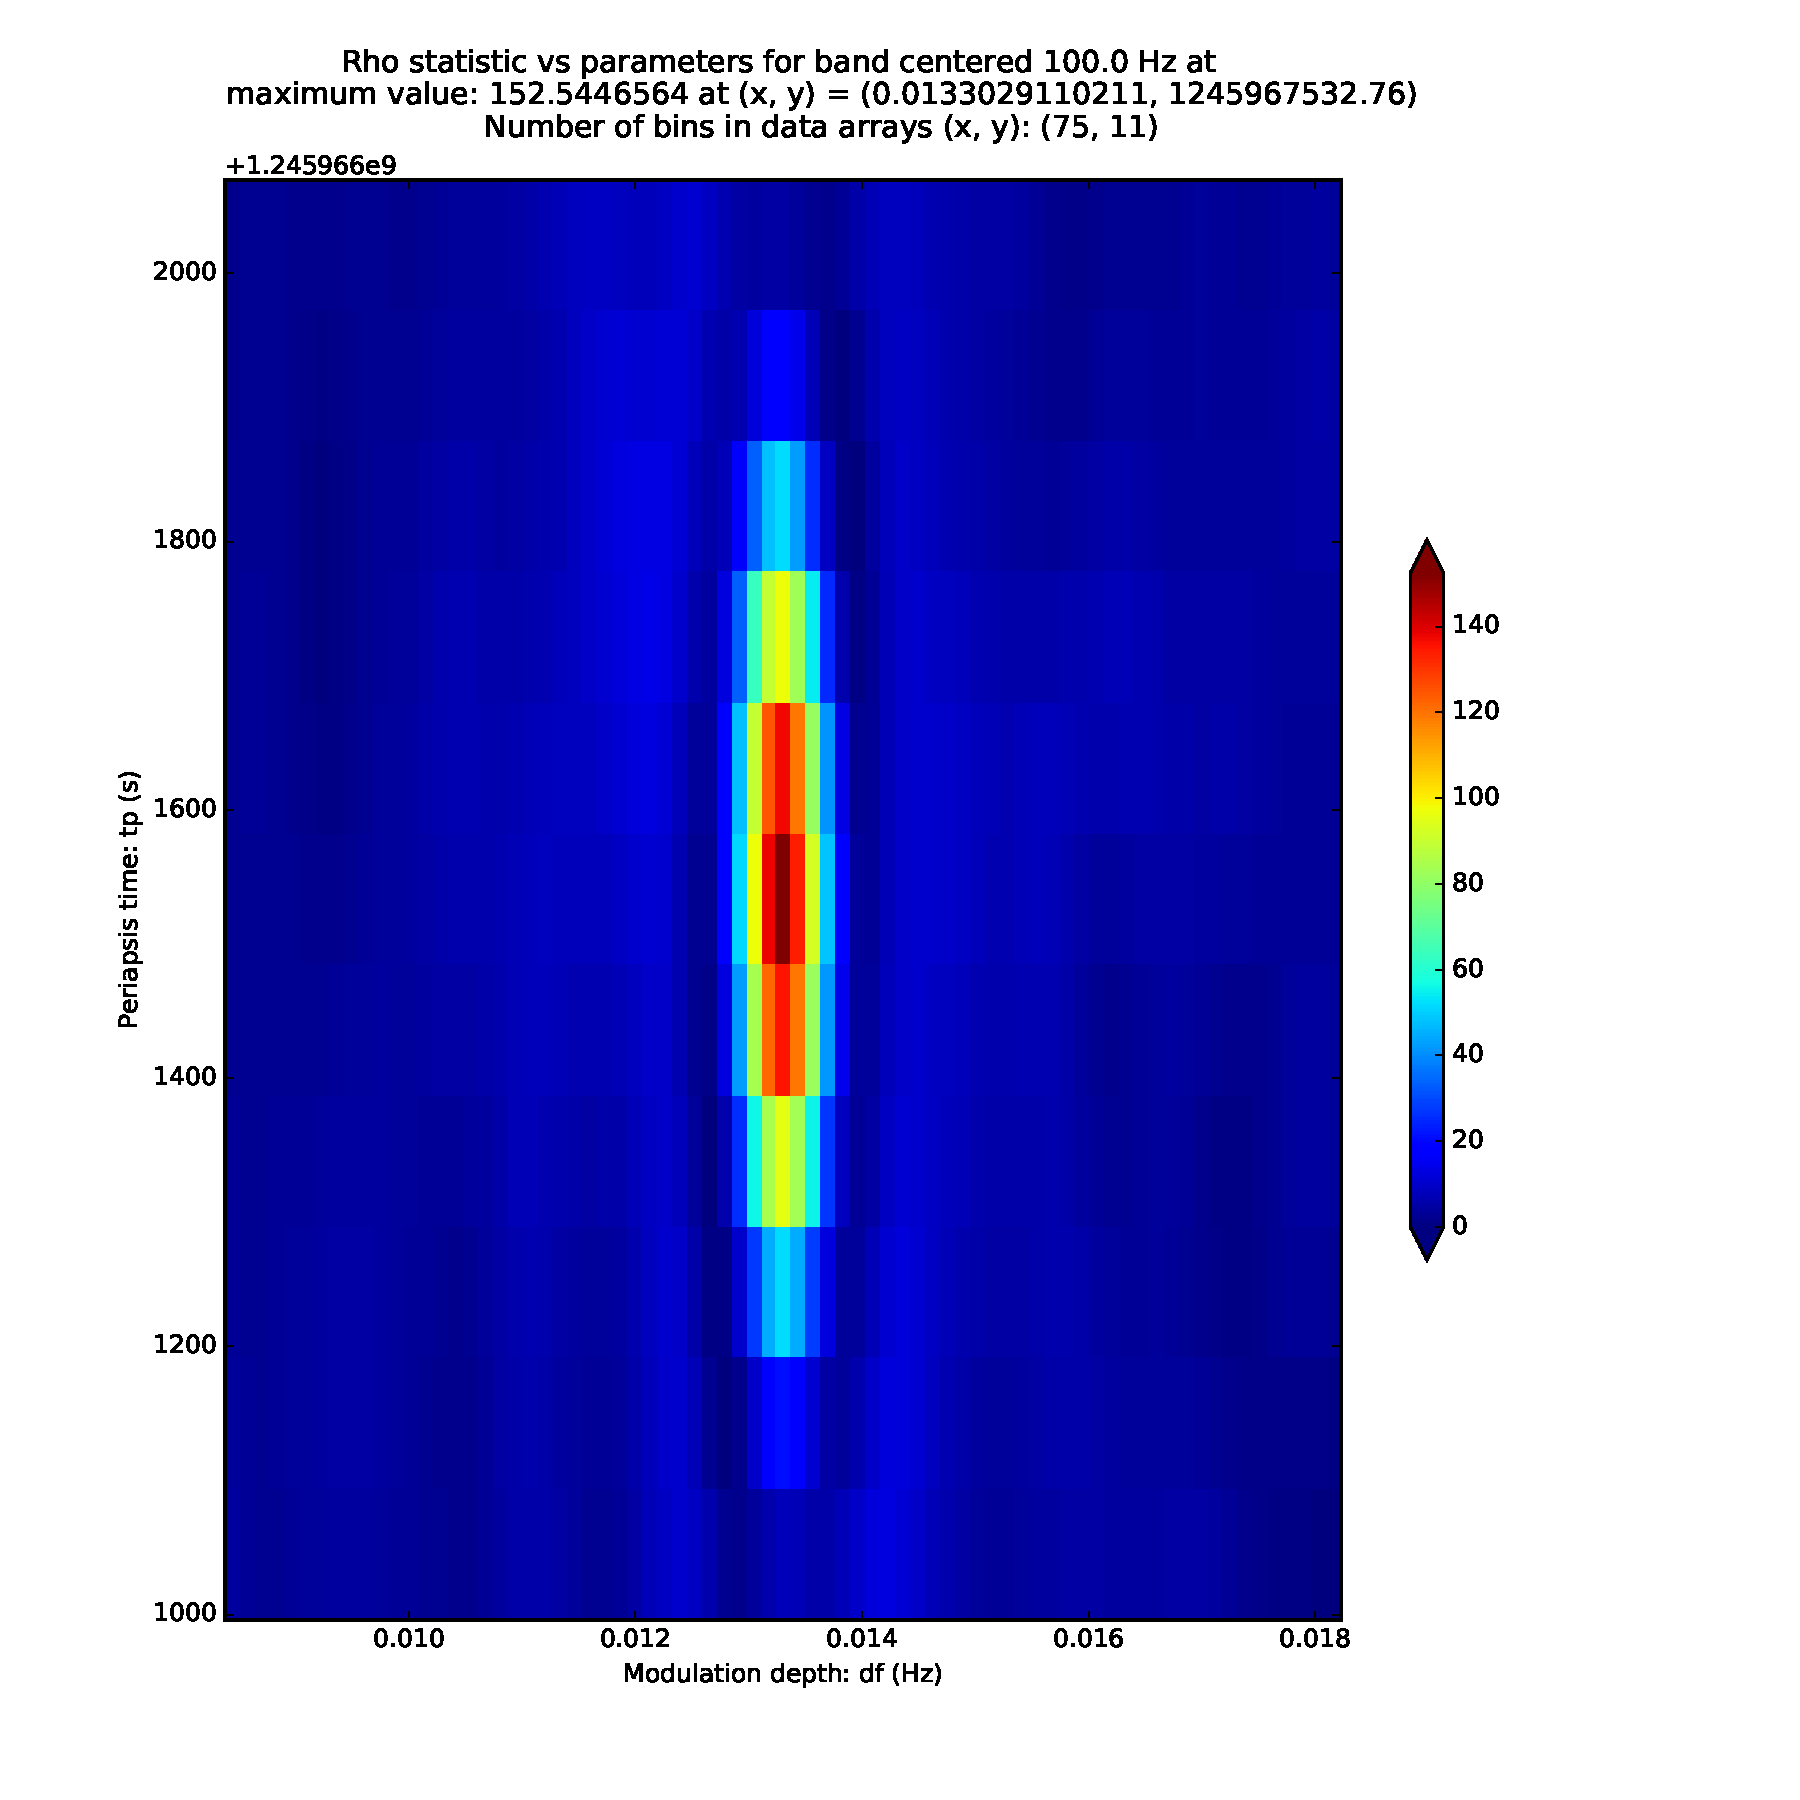
\includegraphics[trim= 0 0 0 0, clip, width=0.40\paperwidth,keepaspectratio]{plots/match-TS/ATresultsR-band-100-0.pdf}
\caption{
\url{<
https://www.atlas.aei.uni-hannover.de/~grant.meadors/LSC/ScoX1/2016/07/21-CrossCorr/match-TS/ATresultsR-band-100.0.pdf
>}
}
\end{figure}

\begin{figure}
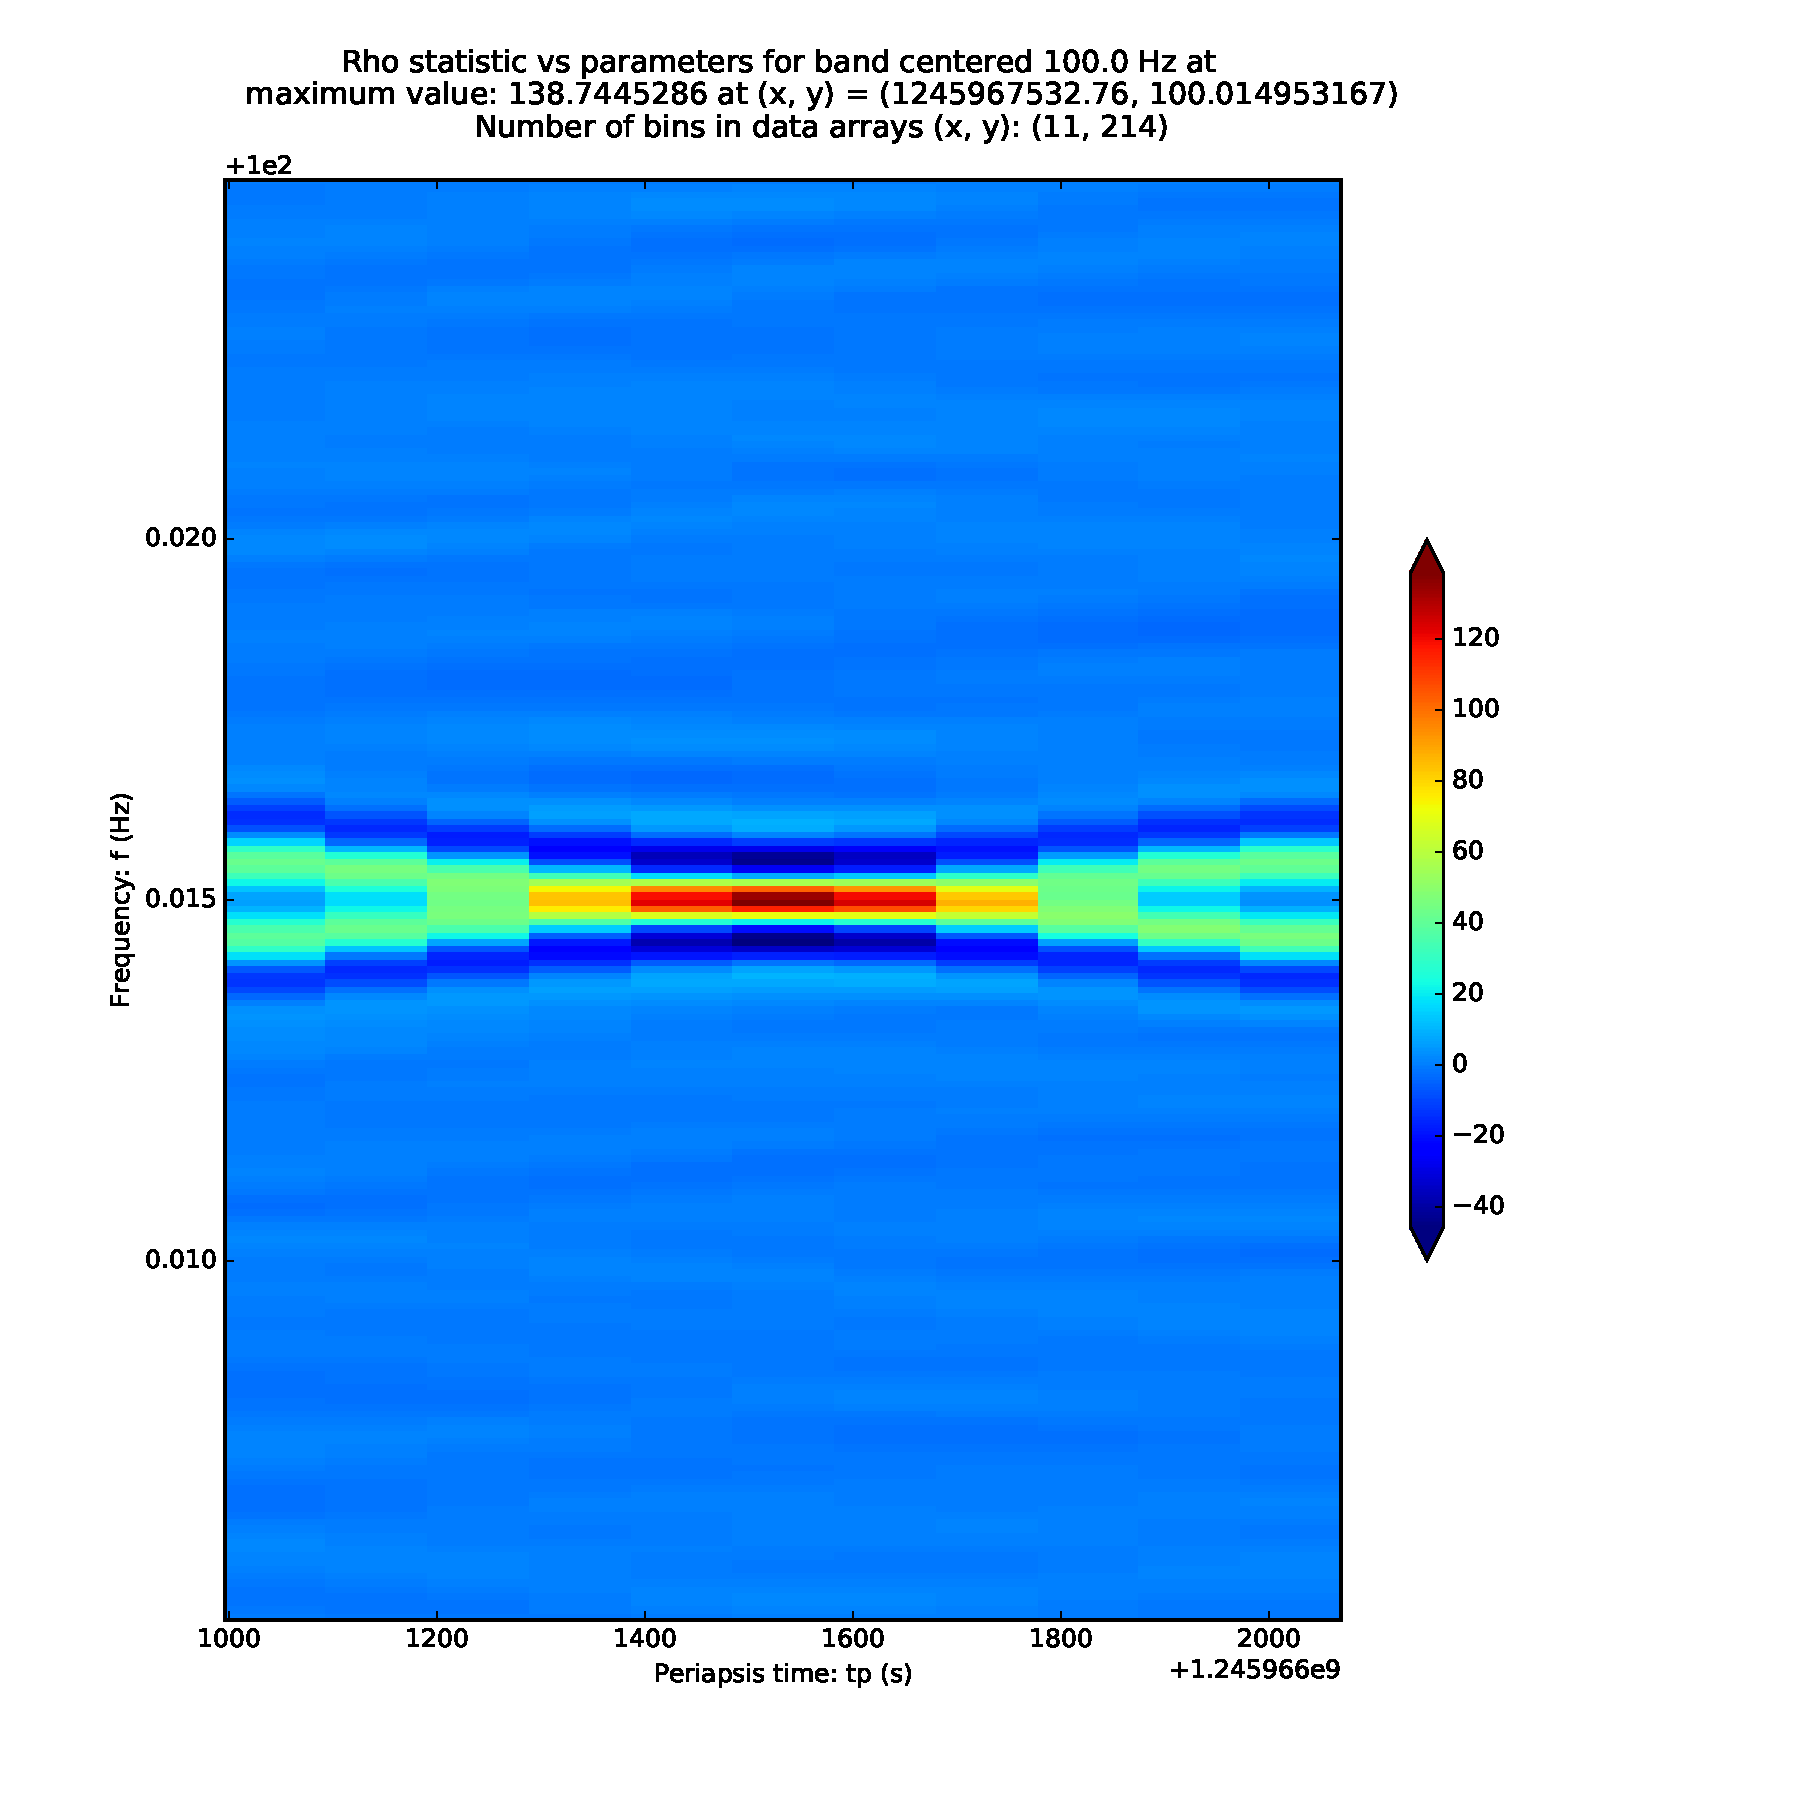
\includegraphics[trim= 0 0 0 0, clip, width=0.40\paperwidth,keepaspectratio]{plots/match-TS/TFresultsR-band-100-0.pdf}
\caption{
\url{<
https://www.atlas.aei.uni-hannover.de/~grant.meadors/LSC/ScoX1/2016/07/21-CrossCorr/match-TS/TFresultsR-band-100.0.pdf
>}
}
\end{figure}


Slices through 5-bin offsets (see "note-on-offsets.txt"), equivalent to

    -frequency = 4.7e-4 Hz,
    -modulation depth = 6.6e-4 Hz,
    -time of ascension = 537 s

show

\begin{figure}
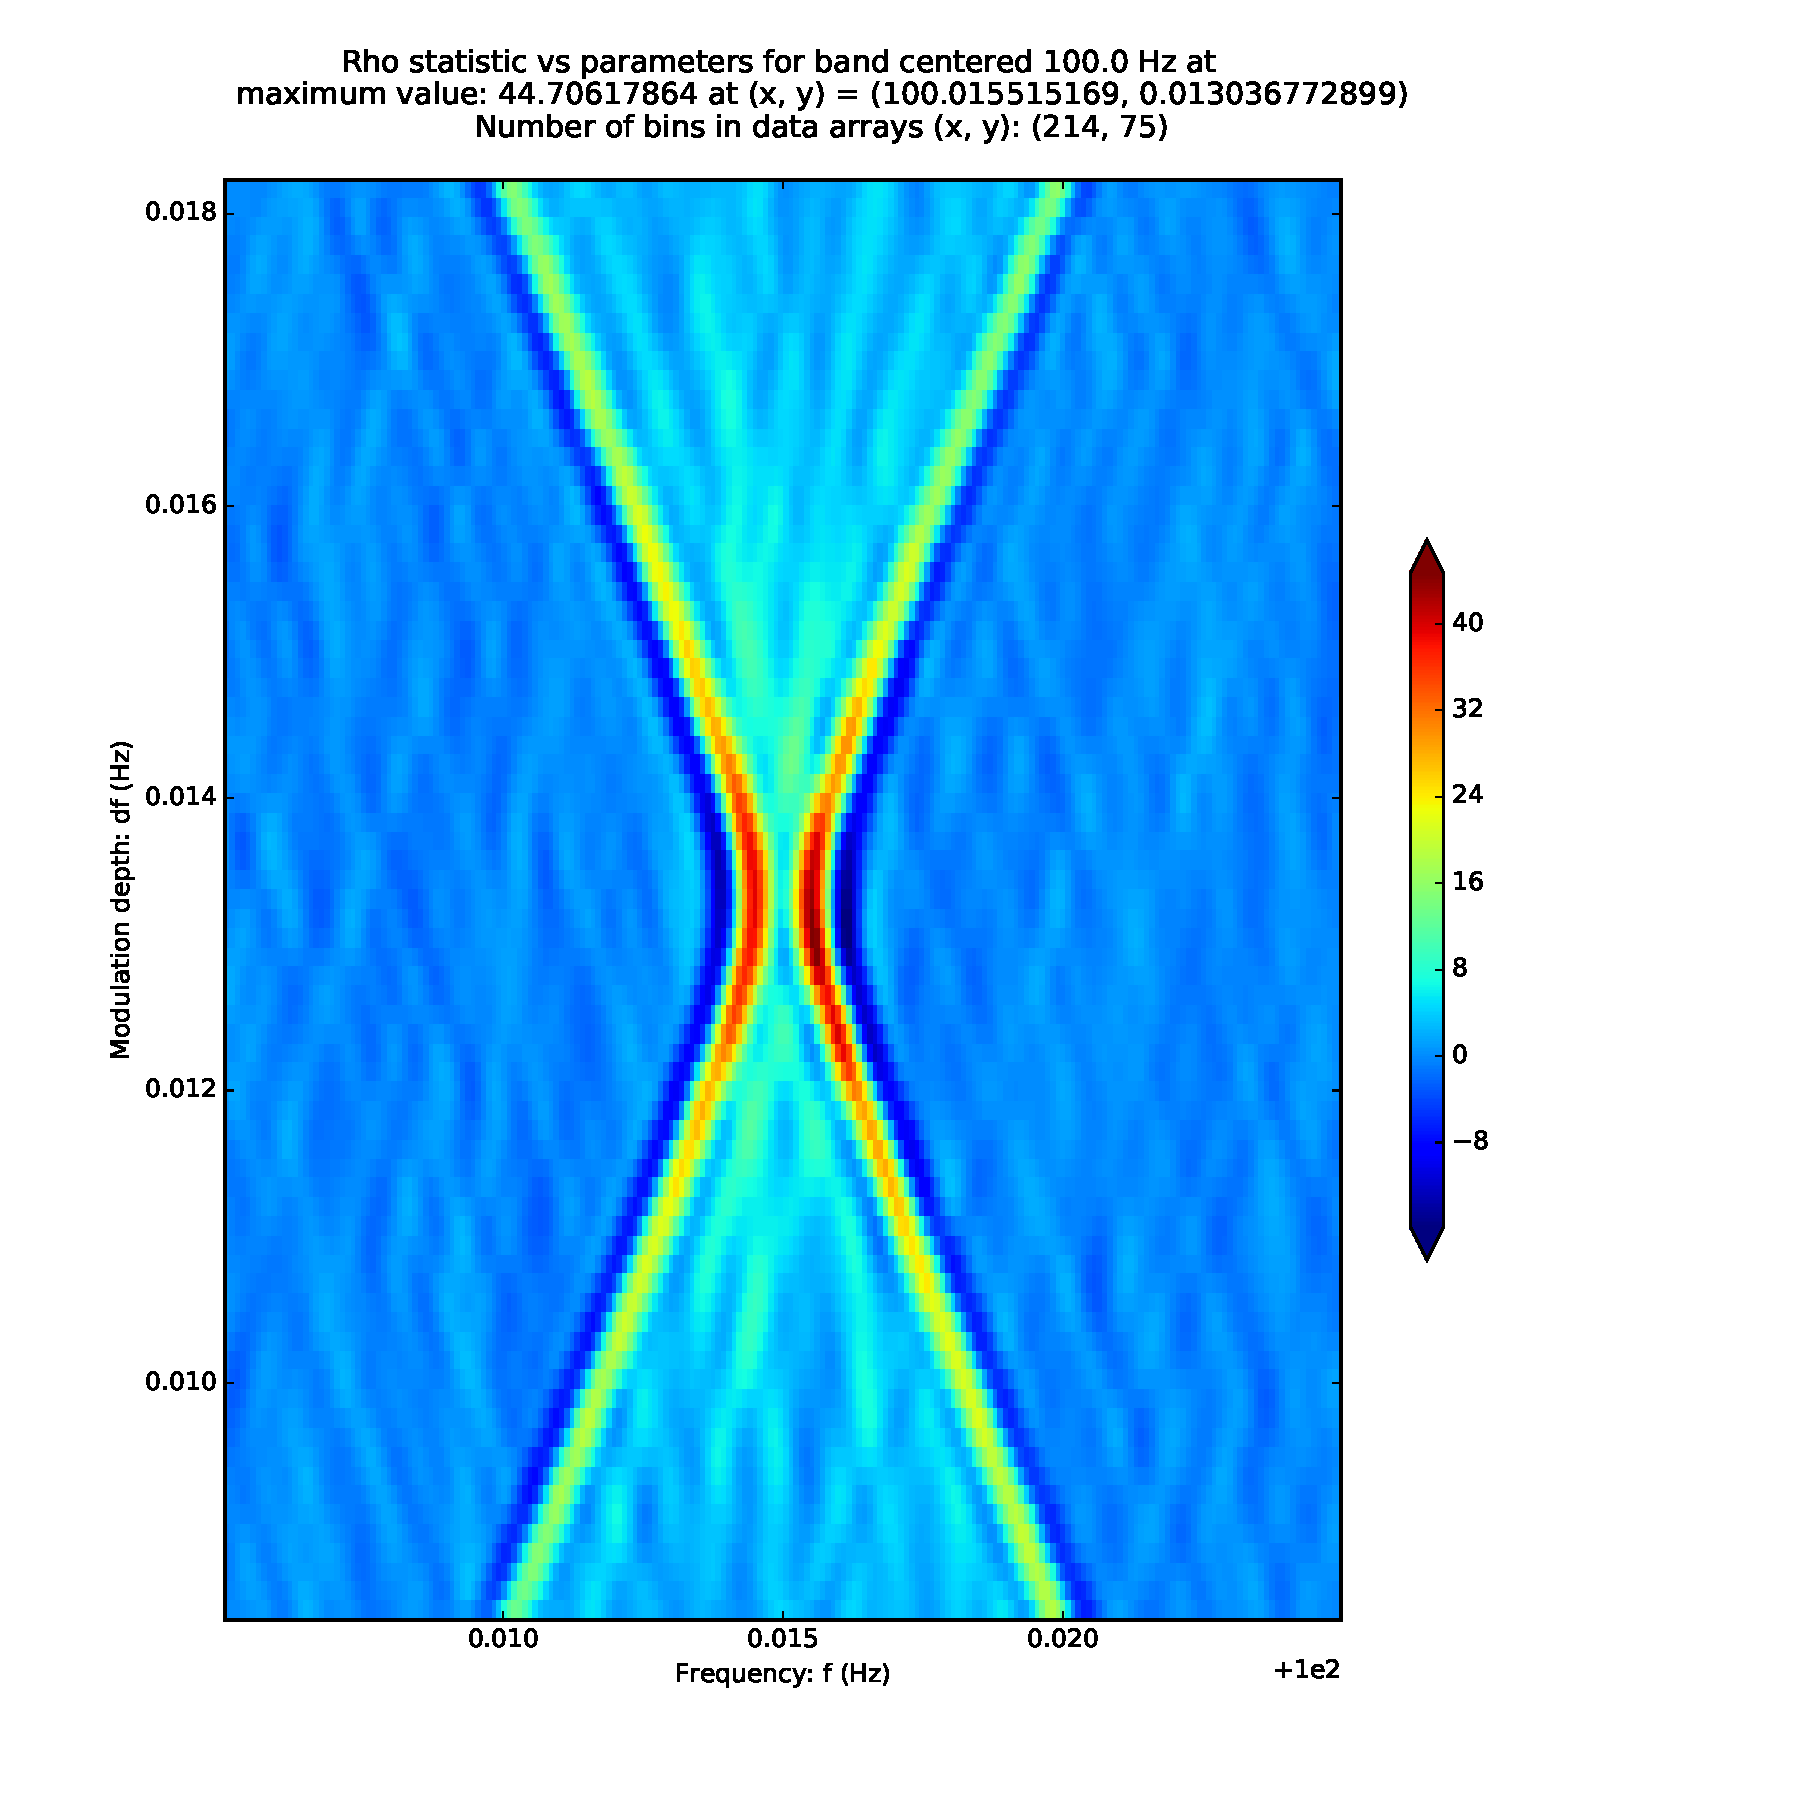
\includegraphics[trim= 0 0 0 0, clip, width=0.40\paperwidth,keepaspectratio]{plots/match-offset-TS/FAresultsR-band-100-0.pdf}
\caption{
\url{<
https://www.atlas.aei.uni-hannover.de/~grant.meadors/LSC/ScoX1/2016/07/21-CrossCorr/match-offset-TS/FAresultsR-band-100.0.pdf
>}
}
\end{figure}

\begin{figure}
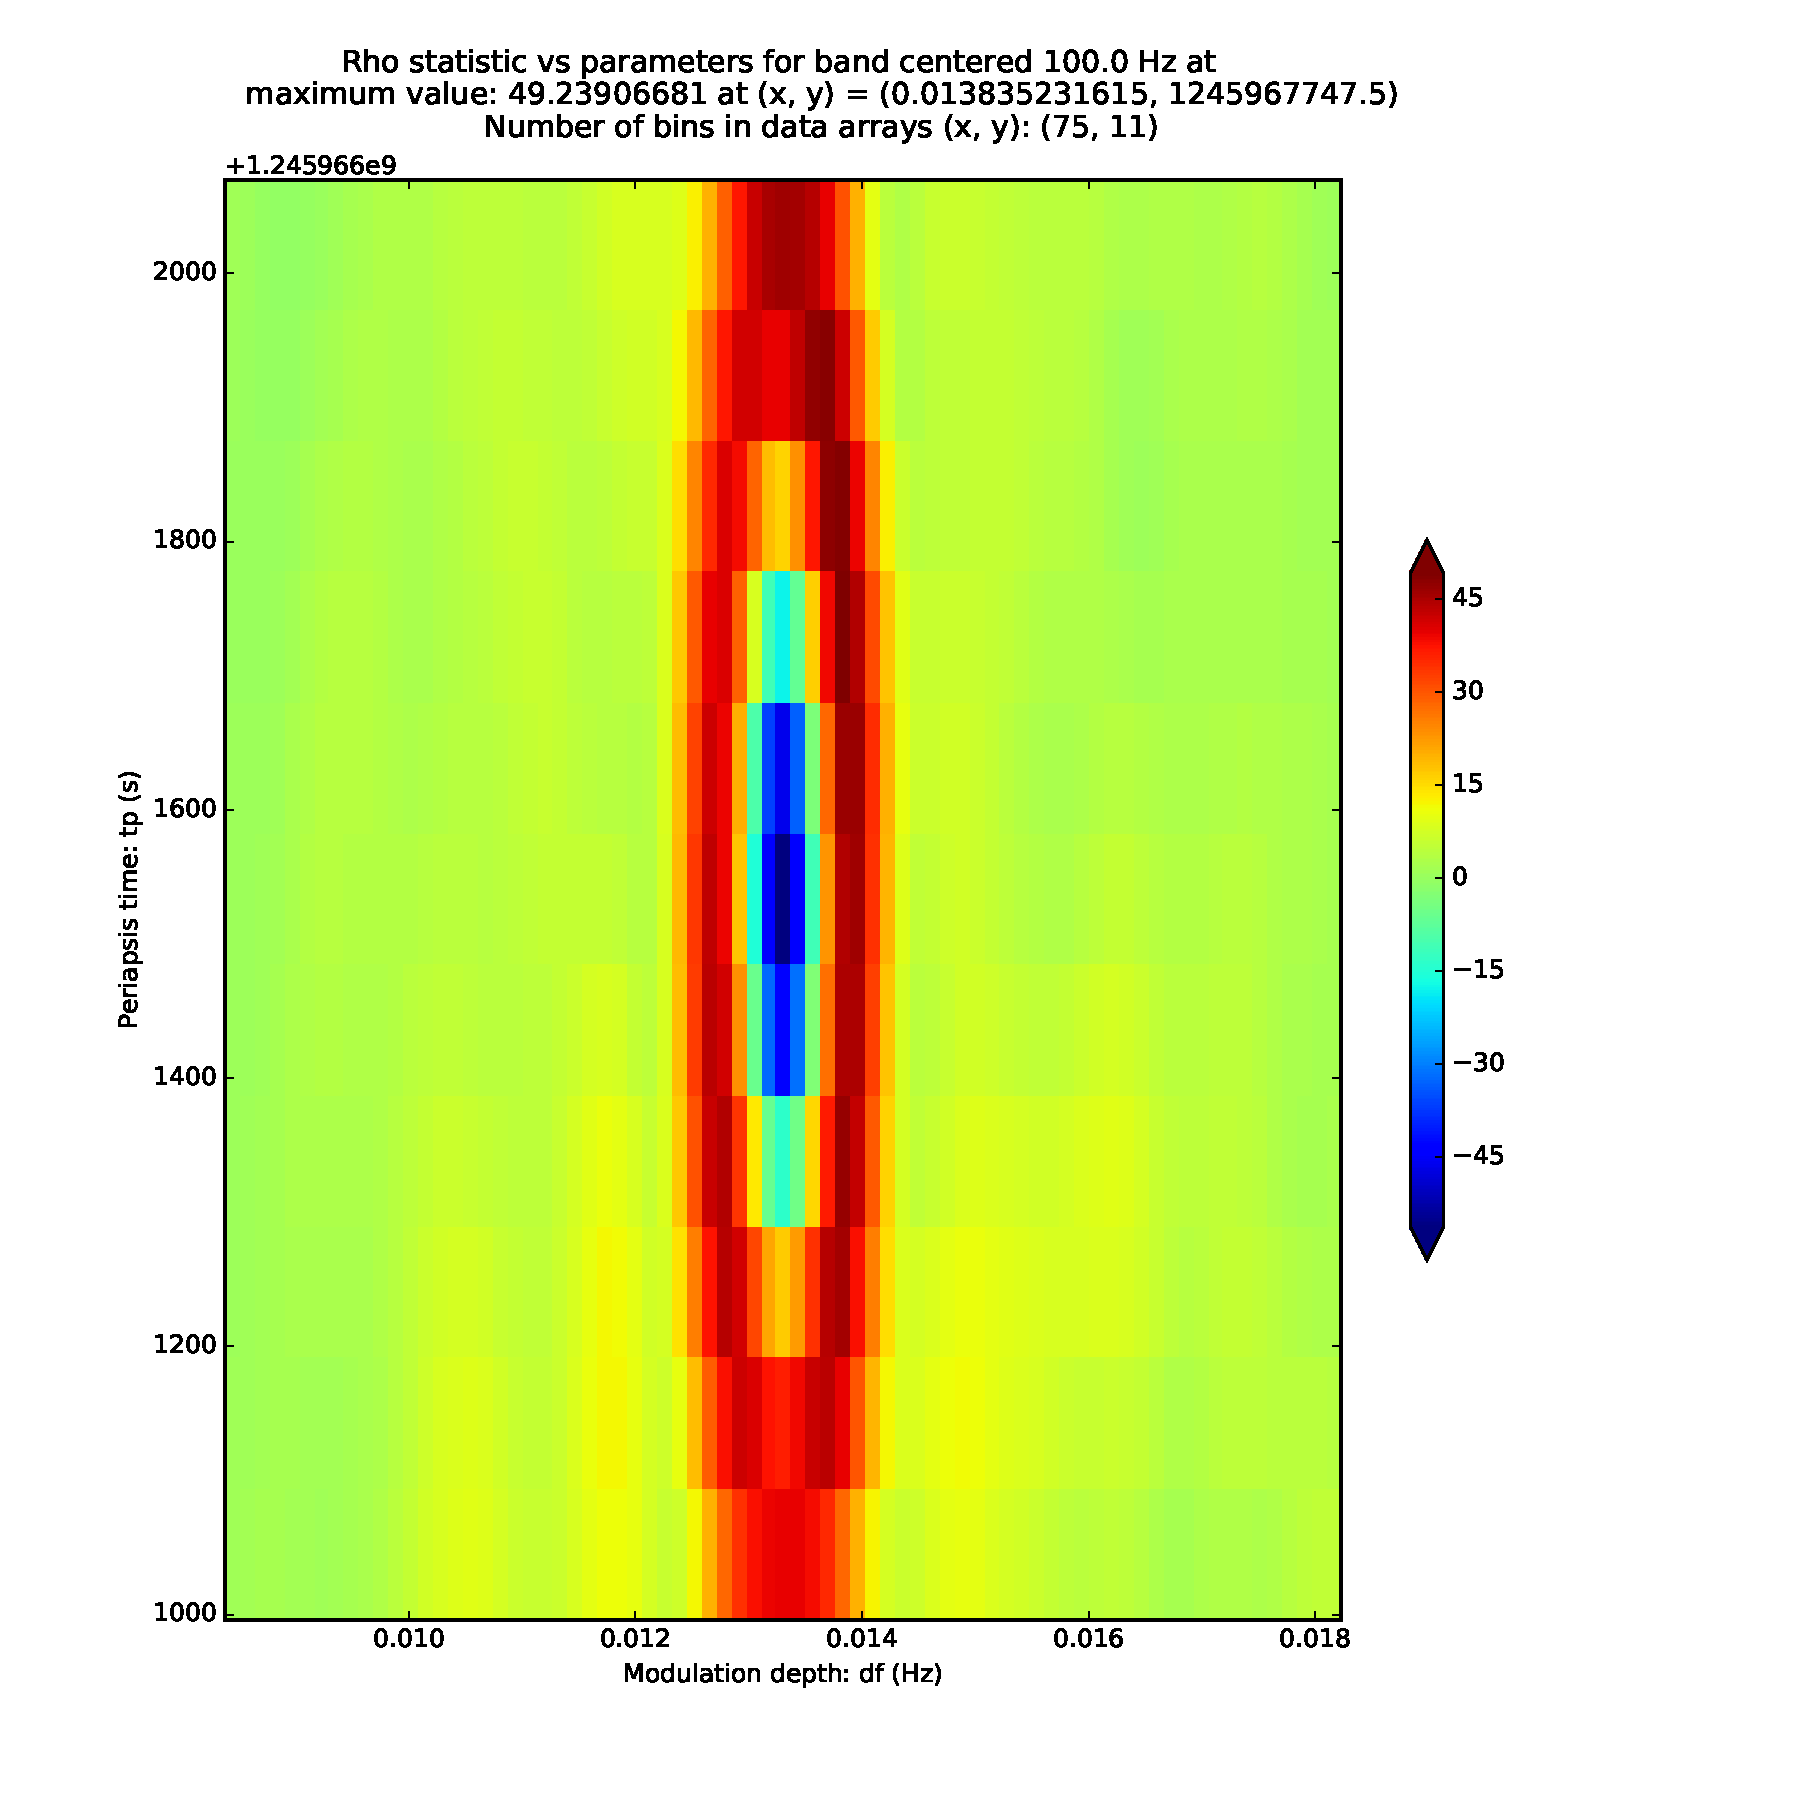
\includegraphics[trim= 0 0 0 0, clip, width=0.40\paperwidth,keepaspectratio]{plots/match-offset-TS/ATresultsR-band-100-0.pdf}
\caption{
\url{<
https://www.atlas.aei.uni-hannover.de/~grant.meadors/LSC/ScoX1/2016/07/21-CrossCorr/match-offset-TS/ATresultsR-band-100.0.pdf
>}
}
\end{figure}

\begin{figure}
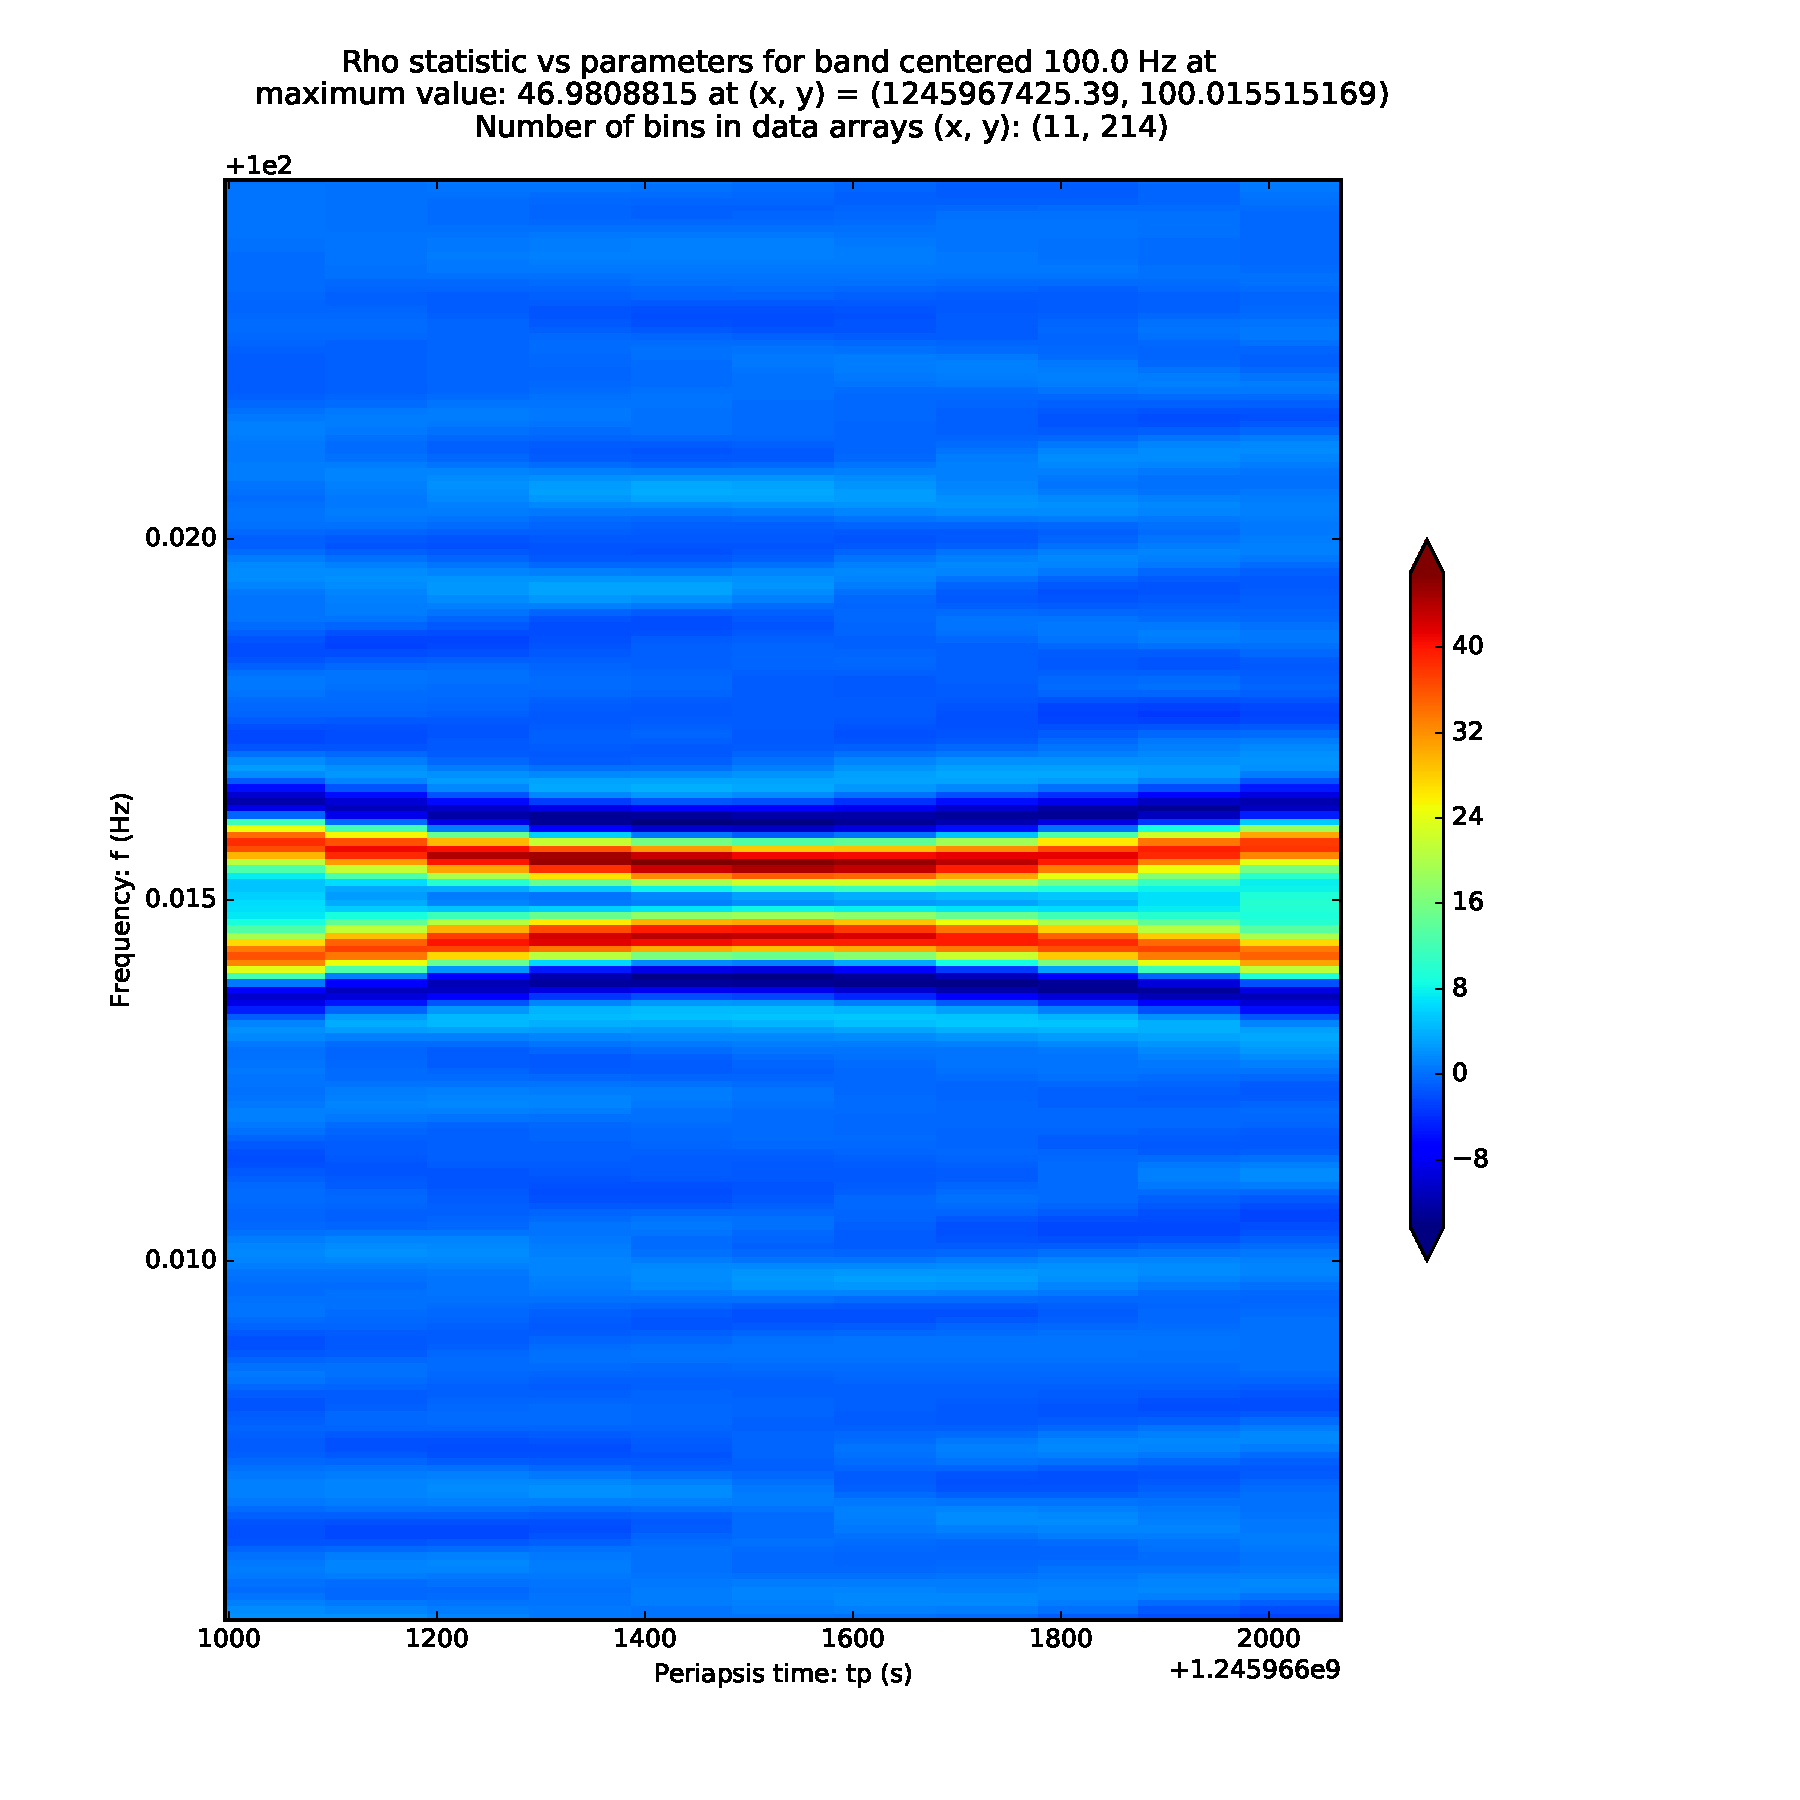
\includegraphics[trim= 0 0 0 0, clip, width=0.40\paperwidth,keepaspectratio]{plots/match-offset-TS/TFresultsR-band-100-0.pdf}
\caption{
\url{<
https://www.atlas.aei.uni-hannover.de/~grant.meadors/LSC/ScoX1/2016/07/21-CrossCorr/match-offset-TS/TFresultsR-band-100.0.pdf
>}
}
\end{figure}

The features of the structure do make sense. As you have probably
figured out, we can predict not only that the slope of d(modulation
depth)/d(frequency) = 1 [equivalently, d(a sin i)/d(frequency) = $P / (2
pi f)]$ in the FA plane,...
    but also that in the TF plane the slope must be max(d(instantaneous
frequency)/dt. With time of ascension $\mathrm{Tasc}$ and $a \sin i$ in seconds ($c$ = 1),

\begin{eqnarray}
  d(\mathrm{instantaneous frequency})/dt
      = d/dt (f0 + (2 pi f0 (a \sin i)/P) \sin[(2 pi/ P)(t - \mathrm{Tasc})])
      = (4 pi^2 f0 (a \sin i)/P^2) \cos[(2 pi/ P)(t - \mathrm{Tasc})])
  \max(d(\mathrm{instantaneous frequency})/dt)
      := (df/dt)
      = 4 pi^2 f0 (a sin i)/P^2
      | f0 = 100.015 Hz, a sin i = 1.44 s, P = 68023.82 s,
      ~= 1.23e-6 Hz / s
      ~= 1 mHz / (1000 s)
\end{eqnarray}

This slope appears to be what we see in the TFresultsR graphs.

The reason for this slope and the X-pattern in the TF plane is best
visualized in the 1st Fourier domain of SFTs (as we think of it in
TwoSpect). There, the signal is a sine-wave with period = P, the orbital
period, centered on f0, with phase determined by Tasc.

If we try an offset template at f' = f+offset, leaving a sin i and Tasc
fixed, it will completely miss the signal. But it can still catch the
RISING edge of the signal's sinusoid if we shift the template orbital
phase: Tasc' = Tasc + $(df/dt)^(-1)$, where $(df/dt)$ ~ 1 mHz/(1000 s) in
our example. Likewise for negative offsets. Or, going the opposite way,
the FALLING edge of the signal can be caught. (signs hopefully right!)

Staying in the 1st Fourier domain, the circle in the AT plane is also
straightforward. For a fixed frequency offset, a template at Tasc', mod
depth = DFobs', can slide the point of contact between the template and
the true sinusoid signal by moving (Tasc', DFobs') in an ellipse. The
respective semi-axes at frequency offset "F\_offset" (F\_offset/$(df/dt)$,
F\_offset).

Conceptual note: we're used to thinking that all the power is in the
"horns", which is true when we sum over SFTs (project the sinusoid's
power onto the frequency dimension), but the instantaneous power in each
bin is relatively constant.

Putting all this together, the CrossCorr structure is a cone given by
the parametric equations [template frequency F', template mod depth
DFobs', template time of ascension Tasc']

\begin{eqnarray}
s \in (-\infty, +\infty), \theta \in [0, 2 pi)
\end{eqnarray}

\begin{eqnarray}
F' - f0                        &=& s\\
DFobs' - (2 pi f0 (a sin i)/P) &=& s * 1 * \cos(\theta)\\
Tasc' - Tasc                   &=& s * (df/dt)^(-1) * sin(theta)
\end{eqnarray}

The middle equation could equivalently be written

\begin{equation}
Asini' - a sin i = s * P/(2 pi f0) * cos(theta)
\end{equation}

And the last expands to

\begin{equation}
Tasc' - Tasc     = s * P^2/(4 pi^2 f0 (a sin i)) * sin(theta)
\end{equation}

There are a few remaining subtleties. For example, $Tasc'$ will have to
start curving to follow large $F'$ offsets -- I'd guess the largest scale
structure in that dimension is actually sinusoidal with period equal to
orbital period $P$ and amplitude $(P/2)$.

To expand in small errors,

\begin{eqnarray}
f &\approx& f0 + err_f + (2pi f0/P)*[
                     (a sin i)*sin(Omega(t-Tasc)) \\
                   &-& err_a * sin(Omega(t-Tasc)) \\
                   &-& (a sin i) * Omega err_t] \\
                   &+& (2pi err_f/P)*(a sin i)*sin(Omega(t-Tasc))
\end{eqnarray}
  (take max)
\begin{eqnarray}
f &\approx& f0 + err_f + (2pi f0/P)*[
                     a sin i \\ 
                   &-& err_a * \\
                   &-& 2 pi (a sin i)/P * err_t] \\
                   &+& O(0)
\end{eqnarray}

Where we see that the ratios of coefficients are the same as above. Call
equal $\Delta f$ errors $eq_f, eq_a, eq_t$:

\begin{eqnarray}
eq_a / eq_f &=& P / (2 pi f0)\\
eq_t / eq_f &=& P^2/(4 pi^2 f0 (a sin i))
\end{eqnarray}

which are the same coefficients as obtained for $(Asini' - a sin i)$ and
$(Tasc' - Tasc)$ above, where we reasoned from the 1st Fourier domain.

Long story short: the structures make sense.

You're welcome to include any of this material on a wiki, though I do
not know where on the wiki to put it. Also, please let me know if this
is old news (and already covered in the iPython notebooks).

My scripts are
    \texttt{wrapCrossCorr.py}
      (wrapper function, itself called as in example-TwoSpect-like.txt)
    \texttt{libCallCC.py}
      (functions for the wrapper)
    \texttt{createHeatmap.py}
      (grapher)

NOTE: ADD material on why there are double-dots at $\pm$ some frequency around the central injection. My guess is that they are at one modulation depth away, and result from being in anti-phase somehow -- but it does not totally make sense. Investigate.

\end{document}
